\documentclass[solution, letterpaper]{cs121}

\usepackage{tikz-qtree}
\usepackage{graphicx}

%% Please fill in your name and collaboration statement here.
%\newcommand{\studentName}{Renzo Lucioni and Daniel Broudy}
%\newcommand{\collaborationStatement}{I collaborated with...}
\newcommand{\solncolor}{red}
\begin{document}

\header{3}{March 15, 2013, at 12:00 PM}{}{}

%%%%%%%%%%%%%%%%%%%%%%%%%%%%%%%%%%%%%%%%%%%%%%%%%%%%
\problem{20} 

%%%%%%%%%%%%%%%%%%%%%%%%%%%%%%%%%%%%%%%%%%%%%%%%%%%%
\problem{25} 

%%%%%%%%%%%%%%%%%%%%%%%%%%%%%%%%%%%%%%%%%%%%%%%%%%%%
\problem{24} 

%%%%%%%%%%%%%%%%%%%%%%%%%%%%%%%%%%%%%%%%%%%%%%%%%%%%
\problem{75}
\begin{enumerate}
	\item 
		\begin{enumerate}
			\item The requested graph is below.
				\begin{center}
				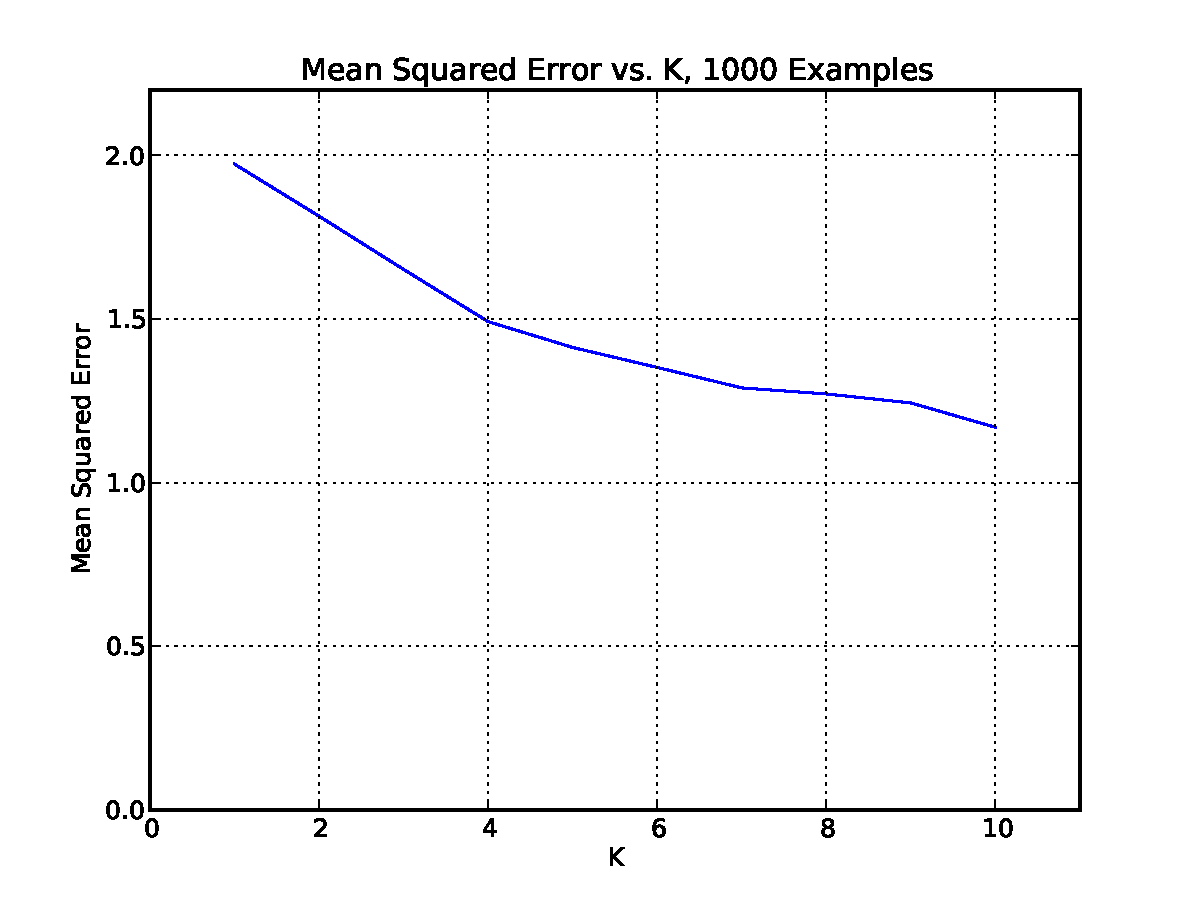
\includegraphics[scale=0.8]{mse-vs-k.pdf}
				\end{center}
			\item If we were to choose the best $K$ for this data based on the plot we generated above, we would choose $K = 8$, since this value of $K$ has a relatively low mean squared error (MSE) without the risk of overcomplicating the model. Choosing a higher value of $K$ will of course result in a lower MSE, but doing this defeats the purpose of clustering, since we are overfitting to the data. In the extreme case, every example in the data will have its own cluster, and the MSE will be 0, but this model does not generalize well.
		\end{enumerate}
	\item
		\begin{enumerate}
			\item The requested table and scatterplots are below. \\
				\begin{center}  
				\begin{tabular}{| c | c | c | c | } \hline
				\multicolumn{2}{| c |}{\emph{min}} & \multicolumn{2}{| c |}{\emph{max}}  \\    \hline         
				Cluster & Instances & Cluster& Instances  \\ \hline
				1 & 1 & 1 & 7\\
				2 & 1 & 2 & 35 \\
				3 & 20 & 3 & 21 \\
				4 & 78 & 4 & 37 \\ \hline
				\end{tabular}
				\end{center}
				\hfill \\
				In the following scatterplots, red circles correspond to cluster 1, blue triangles correspond to cluster 2, green squares correspond to cluster 3, and black stars correspond to cluster 4.
				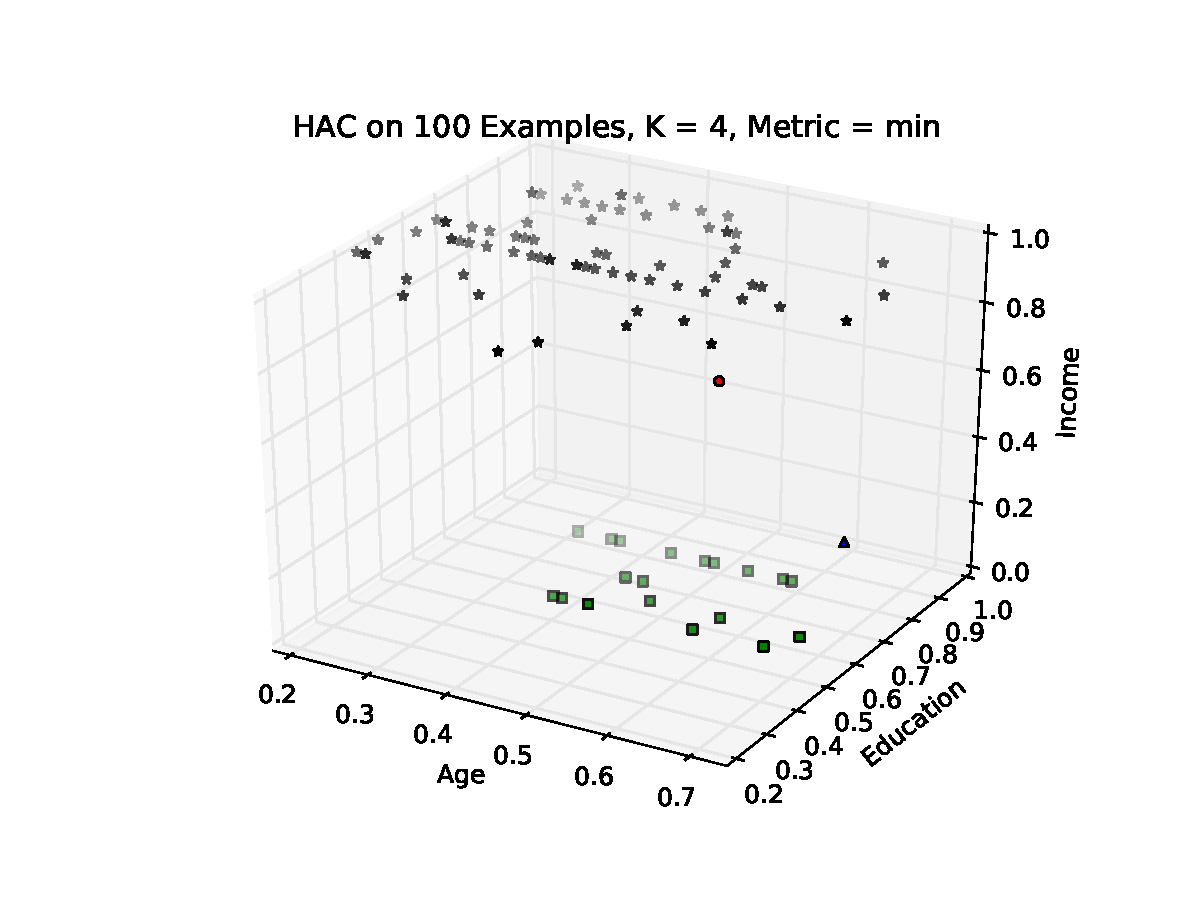
\includegraphics[scale=0.8]{hac-min.pdf}
				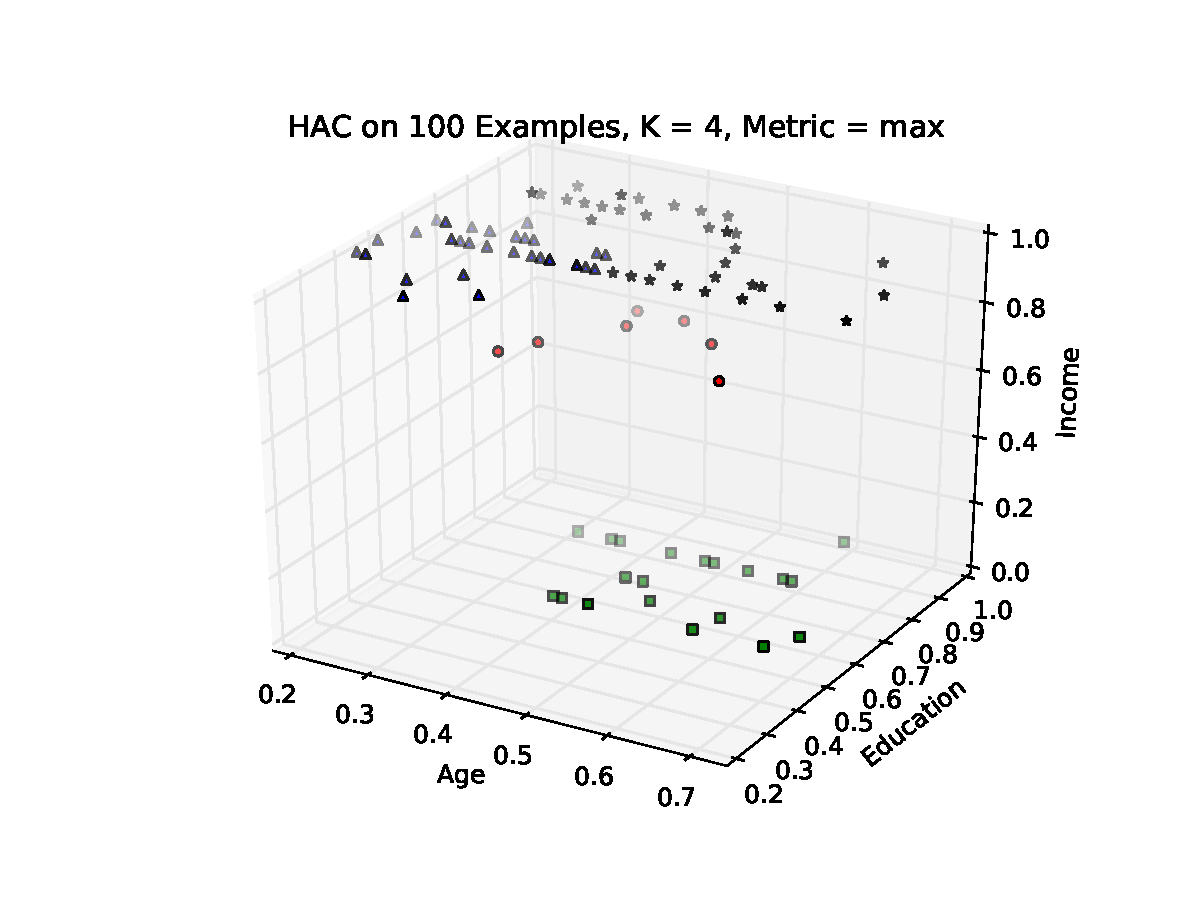
\includegraphics[scale=0.8]{hac-max.pdf} 
				REMARK ON DIFFERENCES AND WHETHER THEY MAKE SENSE GIVEN THE DEF OF THE METRICS
			\item The requested table and scatterplot are below. \\
				\begin{center}  
				\begin{tabular}{| c | c | c | c | } \hline
				\multicolumn{2}{| c |}{\emph{mean}} & \multicolumn{2}{| c |}{\emph{centroid}}  \\    \hline         
				Cluster & Instances & Cluster& Instances  \\ \hline
				1 & 1 & 1 & 1\\
				2 & 26 & 2 & 50 \\
				3 & 50 & 3 & 130 \\
				4 & 123 & 4 & 19 \\ \hline
				\end{tabular}
				\end{center} 
				\hfill \\
				In the following scatterplots, red circles correspond to cluster 1, blue triangles correspond to cluster 2, green squares correspond to cluster 3, and black stars correspond to cluster 4.
				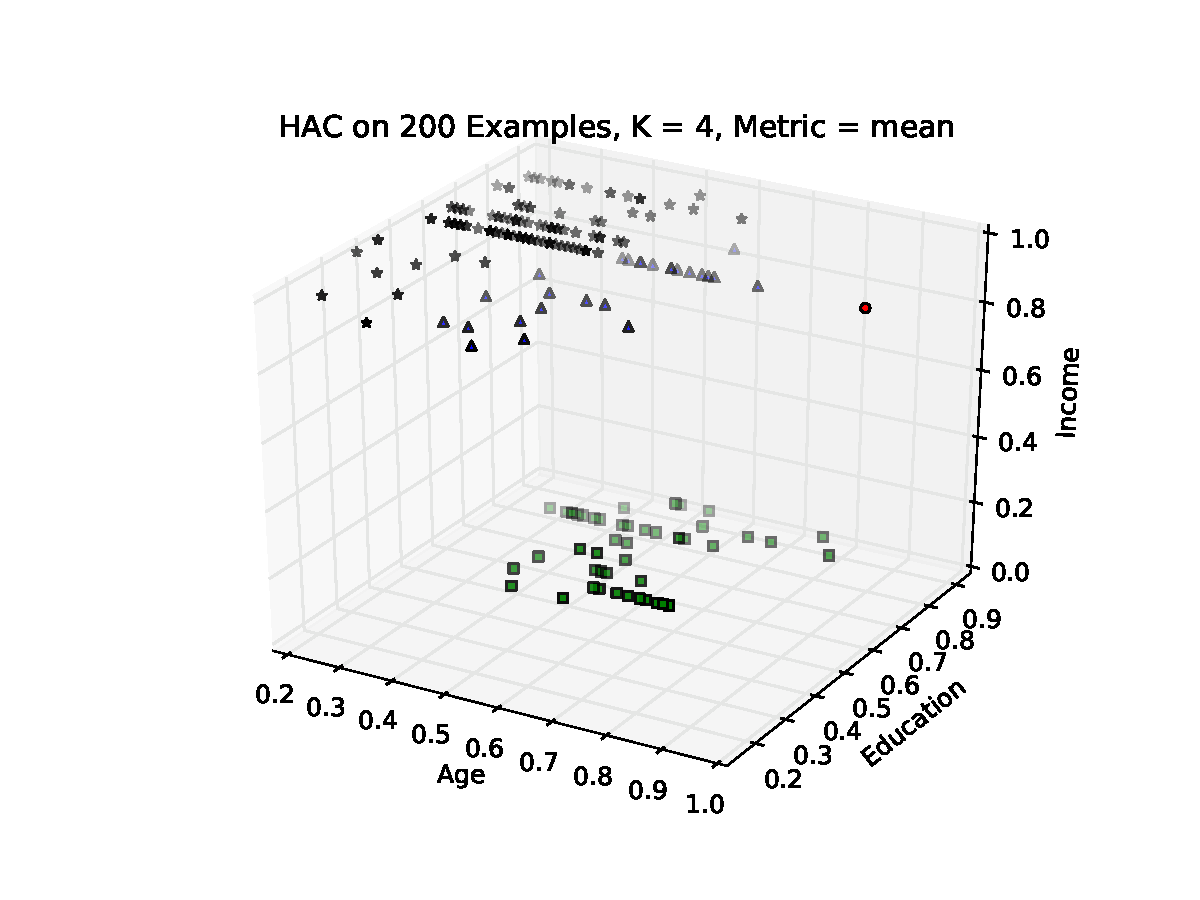
\includegraphics[scale=0.8]{hac-mean.pdf}
				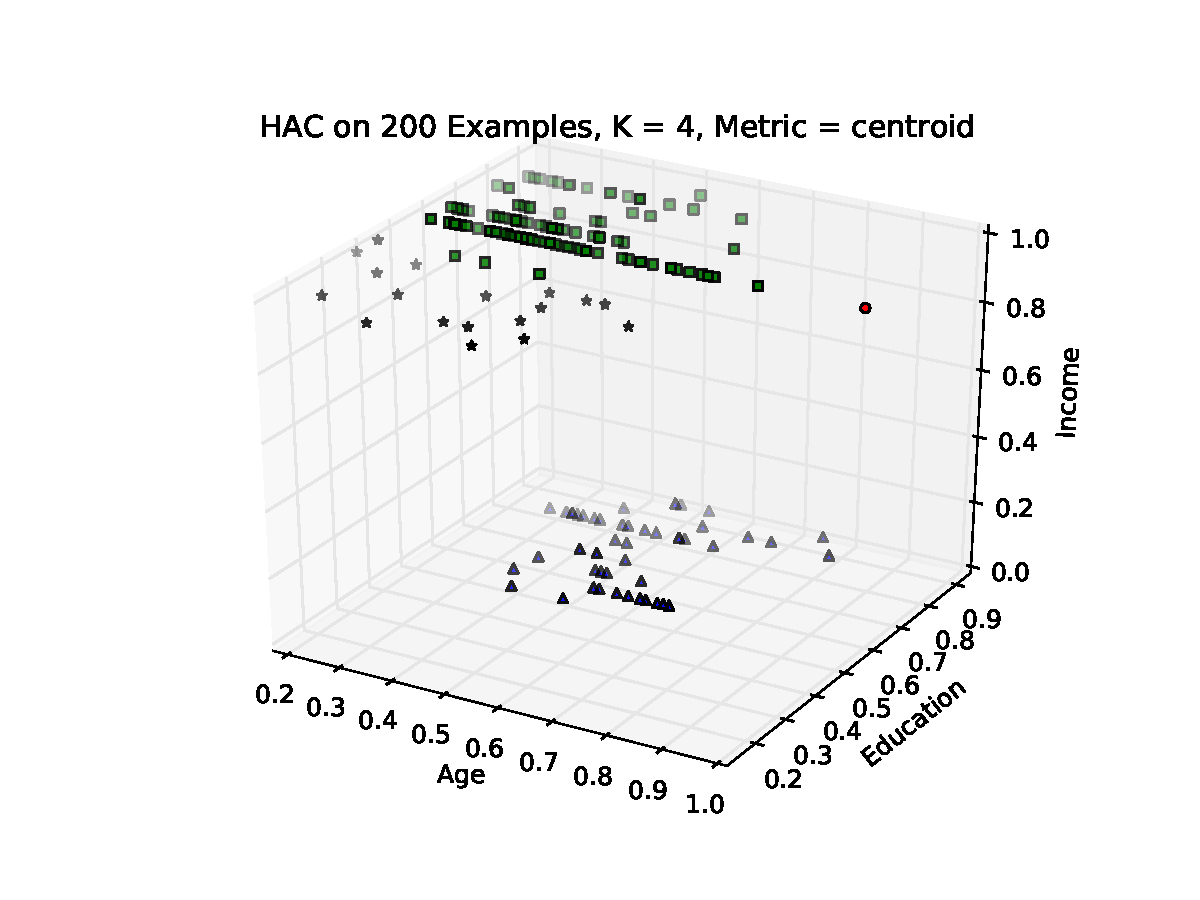
\includegraphics[scale=0.8]{hac-centroid.pdf} 
				REMARK ON DIFFERENCES AND WHETHER THEY MAKE SENSE GIVEN THE DEF OF THE METRICS. Outliers affect the centroid less.

		\end{enumerate}
	\item
\end{enumerate}

\end{document}



